\begin{figure}
  \begin{center}
    \resizebox {.5\columnwidth} {!} {
      \begin{tikzpicture}
        \genealogytree[template=signpost]{
          child{
            g{Agent}
            child{
              g{World Agent}
              child{
                g{Users}
              }
              c{Sources}
            }
            % c[phantom=5em]{aaaaaaa}
            child{
              g{Sky Agent}
              child{
                g{Agent Manager}
                child{
                  g{Agent Manager\\Message Scheduler\\AMMS}
                }
                c{Agent Manager\\Connection Scheduler\\AMCS}
                c{Agent Manager\\Memory Scheduler\\AMME}
              }
            } 
          }
        }
      \end{tikzpicture}
    }
  \end{center}
  \caption{Hierarchy of classes}
  \label{fig:hierarchy}
\end{figure}
\section{Our Model}\label{sec:model}
We use the SLAPP3 platform for agent simulation: this environment provides agent
based protocol in Python 3.
We implemented a hierarchy of agents to manage the different abilities of
each breed.
\\
The class \textit{Agent} is the common and oldest ancestor:
this is required by SLAPP3.\\
Then we have two main classes defining the main branches,
one for the 'real' agents,\textit{WorldAgent}, and another for
the abstract ones, \textit{SkyAgent}.
\textit{WorldAgent} can represent living creatures or tangible objects;
\textit{SkyAgent} is an external agent, living outside the world.\\
Only five breeds of all the implemented classes are produced during
the execution of the program.
This structure allows easy changes and possible future implementations
of the code.

\subsection{WorldAgent}\label{subsec:worldagent}
Two leafs of the tree sprout from this branch: the classes \textit{User}
and \textit{Source}.
The common variables passed by \textit{WorldAgent} are
the vector of mind state and the database of news, used both for memory
and storage. The common members are trivial.
Specifically, the state of mind is a normalized vector of a
specified dimension \texttt{dim} defined inside
\textit{commonVar.py}.

\subsubsection{Source}\label{subsubsec:source}
Sources have a peaked mind state initialized during construction.
The initialization is binary with a number of non-zero values from one to three:
after that, noise is added and the vector is normalized.
Each \textit{Source} has a method, \textit{generateNews}, that can produce
news described with a vector of topics ``near'' the state of the source.
We use near, talking of states, like we talk of geometrical vectors: we will
measure the mind distance with the scalar product of these vectors.

\subsubsection{User}\label{subsubsec:user}
The main class of the program is \textit{User}.
This object contains all the functions to act independently in the world.
We will provide a description of the most important ones.
As mentioned before, a user can compute distance, with the namesake
function, among mind states and between a mind state and a
topic inside news. He can get an opinion on what he sees.
He has a bunch of function to detect who are his neighbors, if they
are sources or users, and if there are only sources around him.
A user can also decide to become active or inactive using internal rules.
He can create or remove an edge between another agent.
Other important users' actions are the way they spread:
\textit{activeDiffusion} and \textit{passiveDiffusion} are the
two functions used to spread news. We will talk about them later.
Finally, an agent can choose how and who manages edges, using
\textit{createEdge} and \textit{deleteEdge}.

\subsection{SkyAgent and AgentManager}\label{subsec:skyagent}
\textit{SkyAgent} has an only child: \textit{AgentManager}: he is
responsible of all the logs.
Other skyagents can be implemented but they are not needed now.

\subsubsection{The Schedulers}\label{subsubsec:schedulers}
There are three leafs out of the \textit{AgentManager's} branch:
\textit{MessageScheduler}, \textit{ConnectionScheduler} and
\textit{MemoryScheduler}. We will refer to them with their
respective abbreviations: \textit{AMMS}, \textit{AMCS} and \textit{AMME}.
The purpose of the logs is to provide a post simulation tool to perform
a complete statistical analysis of the model. 
\begin{itemize}
\item [\textit{AMMS}] This scheduler registers all the spreading during the
  execution. It focuses on the news and registers their creation and
  diffusion, also marking the passive and the active diffusion.
\item [\textit{AMCS}] We can take note of all operations correlated
  to edges: creation, destruction and weight change will
  be registerd in a log file.
\item [\textit{AMME}] This is unlike the other logs. It is not
  called from a user but from the observer.\footnote{TODO specificare
  observer nel protocollo swarm} For every cycle of the program
  this scheduler will print the database of each agent and the activation
  state of anyone.
\end{itemize}

\subsection{Modeling Variables}\label{subsec:variables}
It is not easy to infer a good human mind model. One has to make
a lot of assumptions. For instance, what is important and what is not.
As we said before, the agents live in a network; the connections are the
possibility to communicate and the edge's weight represents the previous
trust.

\subsubsection{Mind State}\label{subsubsec:mindstate}
One way to model mind is to divide it into topics: the number is arbitrary.
The mind now is a vector: each component is a topic. We have choosen
non-negative values as if anyone could be interested in some topic or not.
One can have or not an opinion: there is no distinction between
having a good or a bad point of view.
The initialization of these mind states is binary: the vector starts
with only zeros or ones as said for the sources before. Then rumor is added
and the vector is normalized. We chose to have only one peak each user.

\subsubsection{News}\label{subsubsec:news}
The news is a piece of information that an agent can like or dislike.
For this reason it must be comparable with the mind state.
We have built news as a vector, like the mind state:
its components, geometrically speaking, are near the source's one.
Other important variables for the news are the relevance,
which measures the impact of the news in the world, the
date of creation and the source who made it.

\subsection{Execution}\label{subsec:execution}
Dynamic is regulated by the scheduled structure of SLAPP3. An observer defines
the world time while the model itself provides for a finer structure of
actions. Furthermore, several actions are scripted and interpreted by
the scheduler.

\subsubsection{Observer}\label{subsubsec:observer}
The observer actions used, included in the file \texttt{observerActions.txt},
are \texttt{modelStep}, \texttt{ask\_all}, \texttt{ask\_one},
\texttt{visualizeNet} and \texttt{clock}.
\begin{itemize}
\item [\texttt{modelStep}] is called with its default implementation
\item [\texttt{ask\_all}] calls the \textit{AMME}
\item [\texttt{ask\_one}] calls the finalization of the program. It
  is used in the last line of the file: the line number has to correspond
  to the final clock cycle in order to make this function work.
  To end the execution, log files have to be written, calling
  \texttt{writeLog} which is implemented in each of the \textit{AgentManager's}
  sons. The \texttt{.gml} file of the graph is saved as well as the logs
  in a folder created ad hoc: \texttt{logs}.
  If the execution interrupts or, for some reason, \texttt{ask\_one} is not
  called properly, the files will be saved as well in a temporary folder,
  \texttt{temp}, and the logs will be saved up to the latest
  automatic save (every 1000 lines of log).
\item [\texttt{visualizeNet}] calls the net visualization. The function called
  is \texttt{drawGraph} which is contained in the file \texttt{graph.py}.
  It is also possible to draw the net, to save it in a file or both.
\item [\texttt{clock}] increments the world time.
\end{itemize}

\begin{figure}[htpb]
  \centering
  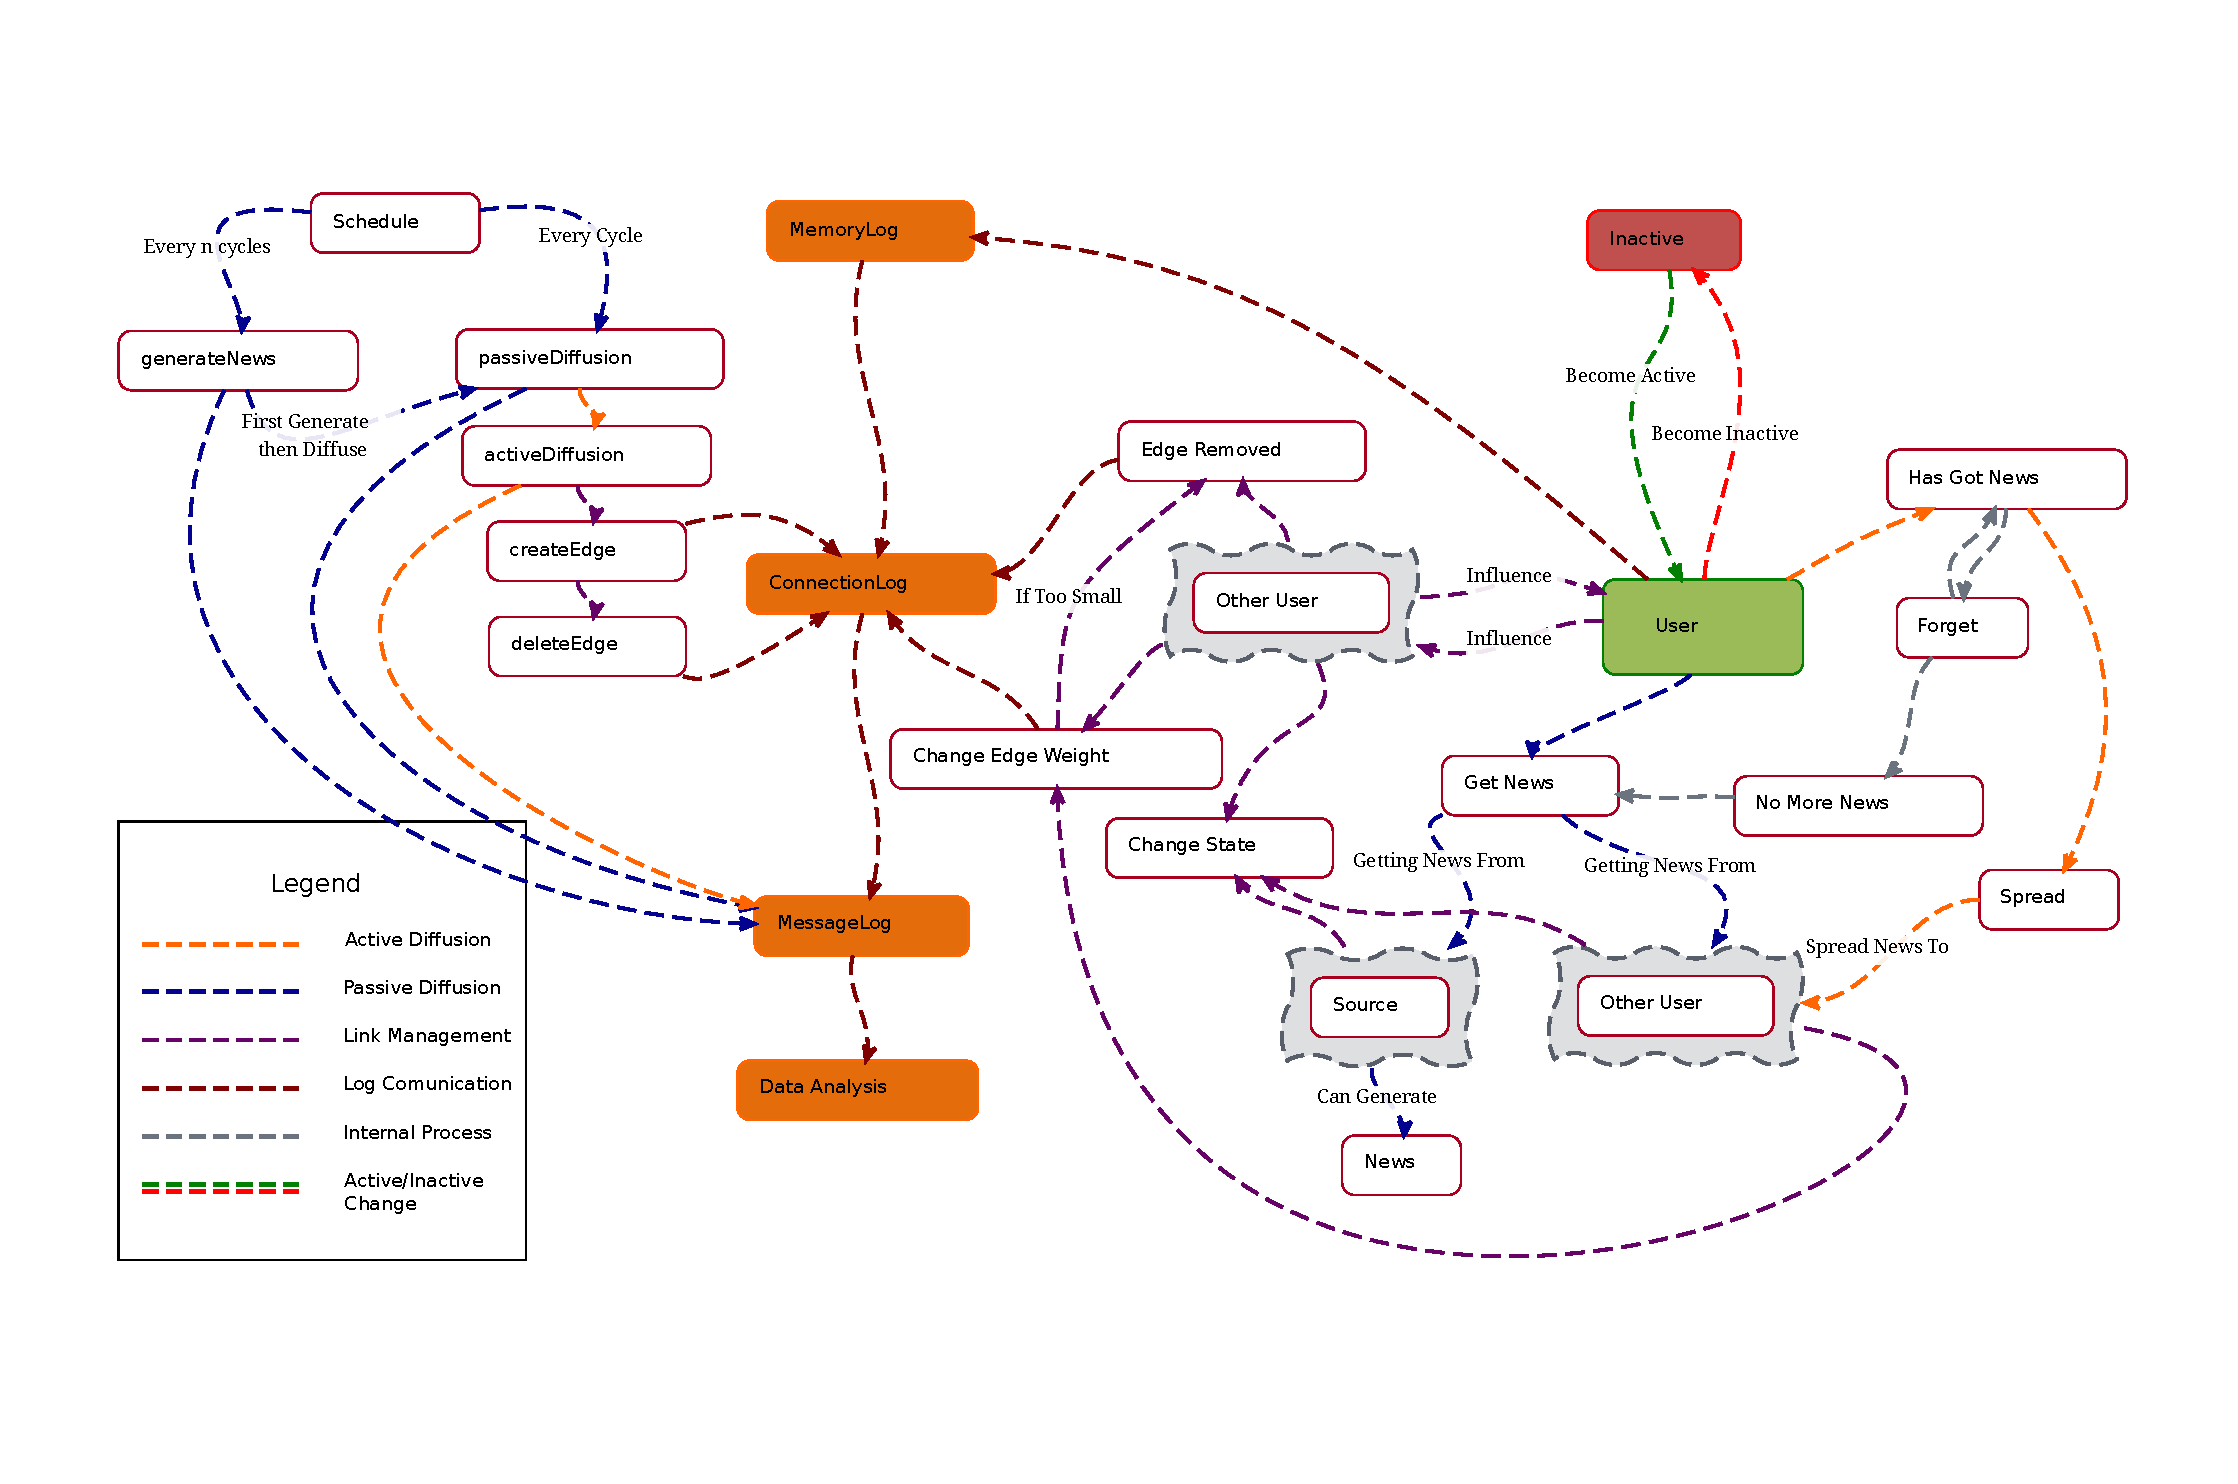
\includegraphics[trim={1.9cm 3cm 1.5cm 2cm}, clip,width=\columnwidth]{img/pdf/mindMap.pdf}
  \caption{Mind map of the model}
  \label{fig:mindmap}
\end{figure}

\subsubsection{Model and Schedule}\label{subsubsec:schedule}
The file \texttt{modelActions.txt} calls the script with
\texttt{read\_script} at every cycle.
The \texttt{reset} and \texttt{move} functions are not implemented
but still called as placeholders.
The file \texttt{schedule.xls} makes three groups of calls:
\begin{itemize}
\item [timestep 1] during the first cycle the program generates news
  contained in the sources;
\item [timesteps 2 - 10000] after news generation and for all
  the execution, users perform passive and active diffusion;
\item [timesteps 10 - 10000] after some time of diffusion the agents start
  to modify the net structure, adding and removing edges with a probability
  of 0.03.
\end{itemize}

\subsection{Overview on simulation: technical difficulties}\label{subsec:overview}
Let us focus on a complete simulation cycle, dealing with some
practical details, while the overview of the main process is given to be
clear to the reader. The figure~\ref{fig:mindmap} explains the main program
workflow during a generic simulation.
From left to right: the schedule runs the main blocks, then the logs start
the acquisition of data, finally we see the actions of a generic agent
during one time step.

\subsubsection{The problem of 'log calling' and 'memory unload'}\label{subsubsec:logcalling}
The breed order creation is log first, then users and finally sources.
We will discuss how and where to call a log during the execution of the program.
As we previously said, logs are agents themselves, not external functions
or tools. The problem is how to call a log at run time; this is solved
only when a single instance of every \textit{AgentManager's} son is
created. Each scheduler, automatically builds himself, during
initialization, inside the \texttt{commonVar.py} file.
It is obvious that this trick will not work for more than one log for breed.
The agent nature of the log is not a bad thing at all because all the logs are
able to manage the memory autonomously: they fill the memory of the machine
up to a limit value of lines and then autosave, appending all the work done
in a temporary file. This allows a limited number of accesses to the disk and
a reasonable amount of memory used during the simulation.

\subsubsection{How to create a graph of agents:
  'further implementation issue'}\label{subsubsec:furtherissue}
The class \textit{WorldAgent} creates the graph during the agent
initializiation. The trick used is clever but can produce some
problems in further implementations. The first agent creates the graph
if he is the first called and if the timestep is 1; all the
agents add themselves into the graph durig their initialization
and the last one creates the edges randomly.
This is a problem if we want to implement a feature for adding nodes.
What we want to avoid is the re-initialization of edges at every new
\textit{WorldAgent} initialization. The simulation works properly if the
number of the agents does not change.

\subsubsection{Determinism and Random}\label{subsubsec:detran}
Agents' actions are deterministic and random.
Let us focus on the action \texttt{createEdge}.
An agent of the breed user can decide to add an edge choosing a node
from the other agents in the net.
He chooses one user randomly and one between his second nearest neighbors,
computing the distance between his mind state and the
possible future linked agent's mind state. To add a bit of randomness
the agent adds all the second nearest neighbors to a list,
sorted by distance and counted with their multiplicity.
Then he chooses randomly from the first ten
elements of the list. Thus we can model deterministic action rules
maintaining the behavior unpredictable.
Other examples of determinism/random can be found in all the spread
and diffusion functions. 

\subsection{What can this model do?}\label{subsec:whatcanthismodeldo}
This model allows to observe different behaviors of agent communities'
interactions.
You can notice the news spreading and the emerging phenomenom of rumor
spreading correlated to it.
Besides, the actions of the agent changing state, while spreading news, bring
out agents' segregation in the network.
All of these effects can be studied also altering agents' memory.
Memory dependency is a new variable introduced as a fundamental
part of the agent's structure.

\subsubsection{News Spreading}\label{subsec:newsspreading}
This model can be used to simulate the spread of one or more news generated
by sources at any cycle of time. The news can also be added or regenerated
every time. It can run for an arbitrary long mind state of agents,
for an arbitrary memory length.
It is written using dictionaries: it provides a very short computational time.
Other mathematical operations are performed including numpy.
Furthertmore it can run very long simulations choosing not to save graphs
and produce logs only for post simulation analysis.

\subsubsection{Segregation}\label{subsec:segregation}
The strength of this model is its abstraction level: it simulates the
spread of a positive normalized vector.
We used it to analyze a group of people sending messages, emails or
talking about news.
It is possible to perform a mind state spreading.
We modeled the spread of a mind state when we used the source as a spreader
of a news, which is near his mind state.
If the assumptions on the vector are good, segregation will emerge from
this model as a common behavior of agent based and network systems.
The segregation, due to different languages, can be modeled as well:
let us think of the mind state as a vector describing the way of speaking.
Each language has a different accent and a different tone: all these things
can be represented as a positive vector.
